\chapter{Implizite Einschrittverfahren}

Steife Systeme treten aber auch in der Modellierung von Reaktionen in der Chemie auf. Als Beispiel soll
eine chemische Reaktion dreier Stoffe $A;B;C$ aus [3] dienen:

\begin{equation*}
	A \rightarrow B, \quad B + B \rightarrow C+ B, \quad B + C \rightarrow A + C
\end{equation*}. 

Die Dynamik der Konzentrationen der einzelnen Komponenten können durch Anfangswertproblem
\begin{align}\label{eq:matrix}
	A:y'_1&= &{}-0.04\cdot y_1  &{}+ 10^4\cdot y_2y_3& & &\\
	B:y'_2&= & 0.04\cdot y_1  &{}- 10^4\cdot y_2y_3& &{}- 3\cdot 10^7y_2^2 &\\
	C:y'_3&= &                  &                  &  & 3\cdot 10^7y_2^2 &\\
\end{align}


mit den Anfangswerten

\begin{equation*}
y_1(0) = 1, y_2(0) = 0, y_3(0) = 0
\end{equation*}  

modelliert werden. Anhand dieses Systems sollen im folgenden steife Differenzialgleichungen untersucht
und ein effizientes numerisches Verfahren entwickelt werden \cite{Prof.Dr.AndreasZeiser.April2021}.

\section{Entwicklung}

Ein allgemeines System von Anfangswertproblemen für eine Funktion y kann als folgendes geschrieben werden:
\begin{equation}
	 y' = f(t,y) ,\quad t \in [a,b],\quad y(a) = y_a 
\end{equation}



Der Wert von y wird näherungsweise an den Zeitpunkten berechnet:
\begin{equation}
	 y^i \approx y(t_i),\quad i = 0,1,\dots,N 
\end{equation}


Das implizite Euler-Verfahren:
\begin{equation}
	 y^{(i+1)} = y^{(i)} + hf\left(t_{i+1},y^{(i+1)}\right) 
\end{equation}


Die implizite Trapezregel:
\begin{equation}
	y^{(i+1)} = y^{(i)} + \frac{h}{2}\left[f\left(t_i, y^{(i)} + f(t_{i+1},y^{(i+1)})\right)\right] 
\end{equation}

\begin{mybox}
\textbf{Aufgabe 1.}	
	Erarbeiten Sie sich Abschnitt 8.4 aus \cite{Atkinson.2004} und fassen Sie in eigenen Worten zusammen, was Sie unter steifen Differenzialgleichung verstehen.
\end{mybox}

	Unter einer steifen Differenzialgleichung versteht man eine Gleichung mit bestimmten numerischen Methoden, die besonders große Störungsfaktoren am Ausgang aufweisen, sofern die Schrittweite nicht allzu klein ausgewählt wird.




\begin{mybox}
	\textbf{Aufgabe 2:}
	Setzen Sie in den Gleichungen des impliziten Euler-Verfahrens und der impliziten Trapezregel
	\begin{equation*}
	\tcbhighmath{\mathbf{y}^{i+1} = \mathbf{y}(i) + \mathbf{z}}  
	\end{equation*}
	
	und formulieren Sie jeweils die Gleichung für  als Nullstellenproblem:
	\begin{equation*}
		\tcbhighmath[]{\mathbf{F}_{\mathrm{euler}}(\mathbf{z}) = 0,\quad \mathbf{F}_{\mathrm{trapez}}(\mathbf{z}) = 0}   
	\end{equation*}
	
\end{mybox}


\begin{equation}
 	y^{(i+1)} = y^{(i)} + hf\left(t_{(i+1)},y^{(i+1)}\right) 
\end{equation}


und die implizite Trapezregel:
\begin{equation}
	 y^{(i+1)} = y_{(i)} + \dfrac{h}{2}\left[f\left(t_i, y^{(i)} + f\left(t_{(i+1)},y^{(i+1)}\right)\right)\right] 
\end{equation}

wir setzen nun
\begin{equation}
	 y^{(i+1)} = y^{(i)} + z 
\end{equation}


in:
\begin{equation}
	 y^{(i)}+ z = y^{(i)} + hf\left(t_i+1,y^{(i)} + z\right) 
\end{equation}



und in:
\begin{equation}
	 y^{(i)} + z = y^{(i)} + \frac{h}{2} \left[f\left(t_i, y^{(i)} + f\left(t_{i+1},y^{(i)} + z\right)\right)\right] 
\end{equation}
ein.

Formulieren wir nun beides als Nullstellenproblem für  erhalten wir
\begin{equation}
	 F_{\mathrm{euler}}(z) = z - hf(t_{i+1}, y^{(i)} + z) = 0 
\end{equation}

und 
\begin{equation}
F_{\mathrm{trapez}}(z) =  z - \frac{h}{2} \left[f\left(t_i, y^{(i)} + f(t _{i+1},y^{(i)} + z)\right)\right] = 0
\end{equation}

\begin{mybox}
\textbf{Aufgabe 3. :}
Bestimmen Sie die Jacobi-Matrizen $D\textbf{F}_{\mathrm{euler}}$ und $D\textbf{F}_{\mathrm{trapez}}$ von $\textbf{F}_{\mathrm{euler}}$  und $\textbf{F}_{\mathrm{trapez}}$  in Abhängigkeit von $D_yf$, d.h. der Jacobi-Matrix von $f$ bezüglich $y$ .
\end{mybox}

\begin{equation}
	 D\cdot F_{\mathrm{euler}}(z) = D\cdot z - h\cdot D_y\cdot f\left(t_{i+1}, y^{(i)} + z\right) 
\end{equation}


für das implizite Euler-Verfahren und
\begin{equation}
	 D\cdot F_{\mathrm{euler}}(z) = \frac{h}{2}\cdot \left[D_{y}\cdot f\left(t_{i+1}, y^{(i)}) +  h\cdot D_y f(t_{i+1}, y^{(i)} + z)\right)\right] - D\cdot z 
\end{equation}


für das implizite Trapez-Verfahren,

wobei 
\begin{equation}
	D, f =
\begin{bmatrix}
	\frac{\partial f_1 }{\partial y_1} & \frac{\partial f_1 }{\partial y_2} & ... & \frac{\partial f_1 }{\partial y_n} \\
	\frac{\partial f_2 }{\partial y_1} & \frac{\partial f_2 }{\partial y_2} & ... & \frac{\partial f_2 }{\partial y_n} \\
	... & ... & ... & ... \\
	\frac{\partial f_n }{\partial y_1} & \frac{\partial f_n }{\partial y_2} & ... & \frac{\partial f_n }{\partial y_n} 
\end{bmatrix} 
\end{equation}


und 
\begin{equation}
	Dz =
\begin{bmatrix}
	1 & 0 & ... & 0 \\
	0 & 1 & ... & 0 \\
	... & ... & ... & ... \\
	0 & ... & 0 & 1 
\end{bmatrix}  
\end{equation}

\begin{mybox}
	\textbf{Aufgabe 4. :}
	Implementieren Sie die folgenden zwei Routinen. Verwenden Sie für die Jacobi-Matrix $J$ dünnbesetzte
	Matrizen.
\end{mybox}

\begin{figure}[htb]
	\lstinputlisting[style=Matlab-editor]{Matlab_files/F_euler.m}
\end{figure}
\begin{figure}[htb]
	\lstinputlisting[style=Matlab-editor]{Matlab_files/F_trapez.m}
\end{figure}
\clearpage
\begin{mybox}
	\textbf{Aufgabe 5. :}
	Implementieren Sie die Löser aufbauend auf den Routinen des letzten Abschnitts und des Newton-Verfahrens aus der Belegarbeit. Als Startwert der Newtoniteration wählen Sie für $z$ den Nullvektor.
\end{mybox}

\begin{figure}[htb]
	\lstinputlisting[style=Matlab-editor]{Matlab_files/impl_euler.m}
\end{figure}
\begin{figure}[htb]
	\lstinputlisting[style=Matlab-editor]{Matlab_files/impl_trapez.m}
\end{figure}
\clearpage

\begin{mybox}
	\textbf{Aufgabe 6. :}
	Bestimmen Sie wie in den Übungsblättern anhand des Anfangswertproblems $ y' = -y $ mit Anfangsbedingung $ y(0) = 1 $ auf dem Intervall $ [0,1] $ graphisch die Ordnung der beiden Verfahren.
\end{mybox}

\begin{figure}[h]
	\centering
	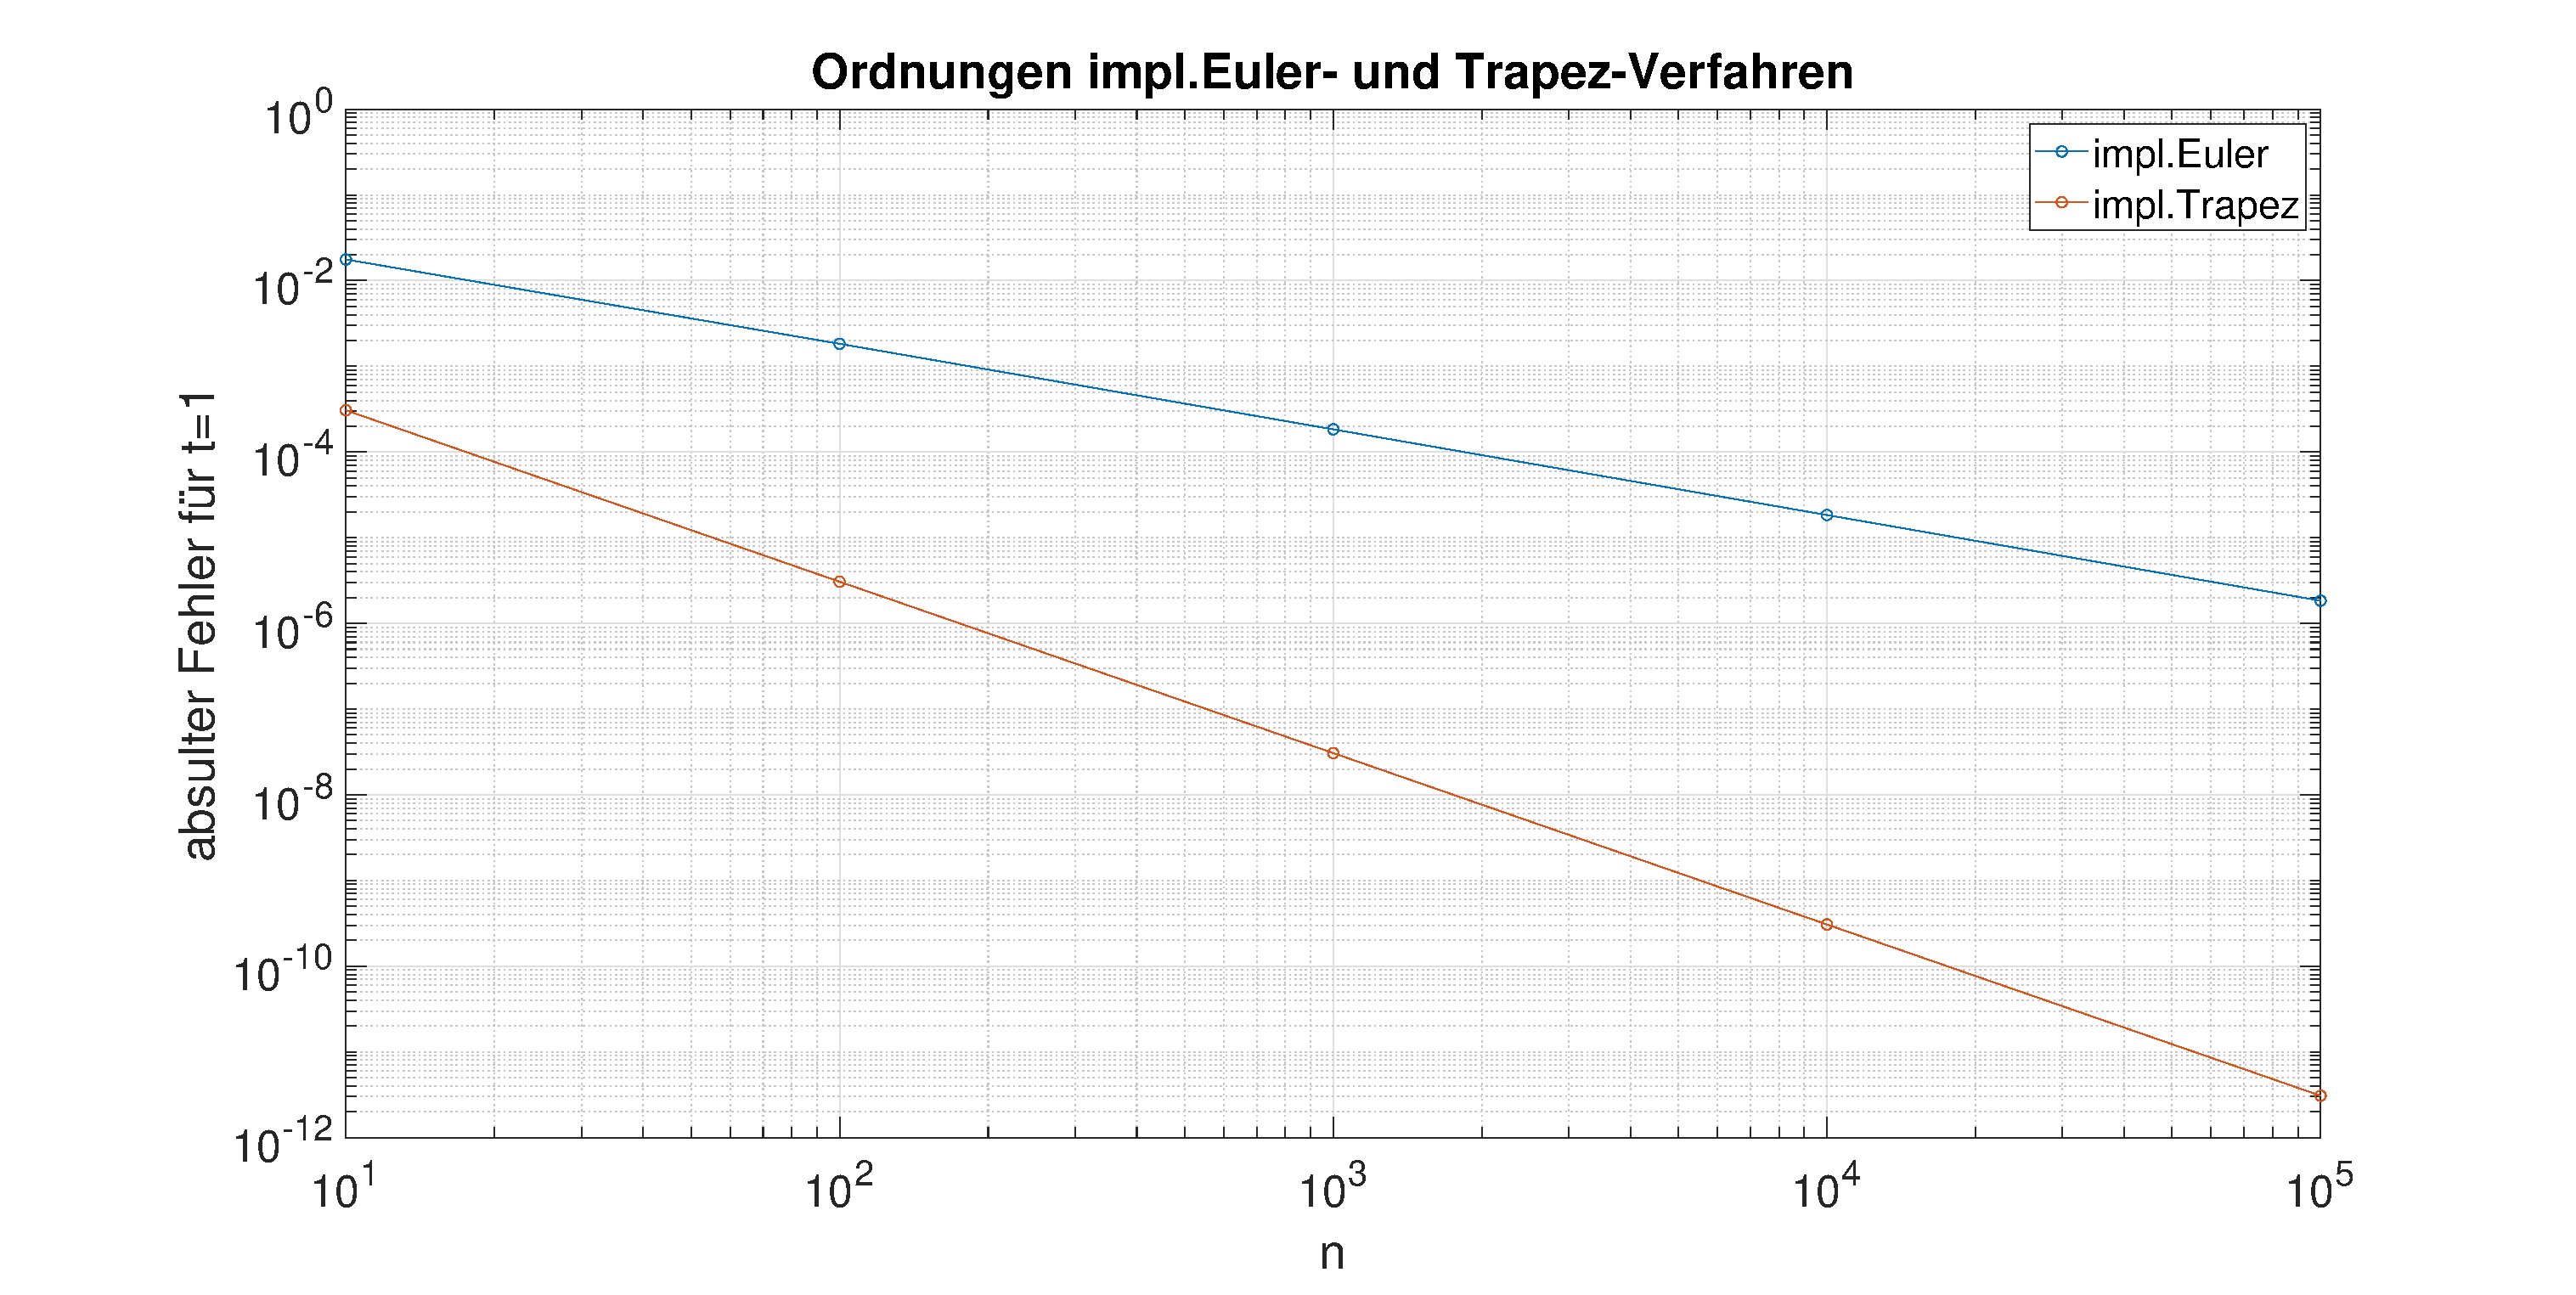
\includegraphics[width=1\textwidth]{figures/Impl._3_1_6/Ordnungen_E_T}
	\caption{die Ordnungen von impliziten Euler- und Trapez-Verfahren}
\end{figure}


\clearpage


\begin{mybox}
	\textbf{Aufgabe 7. :} Testen Sie Ihre Routine anhand eines geeigneten nichtlinearen, zeitabhängigen Systems von Anfangswertproblemen.
\end{mybox}

\begin{equation}
y^{\prime } =\left\lbrack \begin{array}{c}
	-2t\cdot y_1 -3y_2 \\
	2y_1 +{t^2 \cdot \;y}_2 
\end{array}\right\rbrack \;\mathrm{mit}\;y\left(0\right)=\left\lbrack \begin{array}{c}
	3\\
	1
\end{array}\right\rbrack ,t=\left\lbrack 0,2\right\rbrack ,
\end{equation}

Als Test für das System wird folgendes Gleichungssystem(nichtlinear) entwickelt:
\lstinputlisting[style=Matlab-editor,caption={Test zum Lösen von nichtlinearen, zeitabhängigen System von Anfangswertproblemen}]{Matlab_files/Test_3_1_7.m}


\section{Anwendung}
\begin{mybox}
	\textbf{Aufgabe 1. :} Formulieren Sie Gleichung (9) als System der Form (11) mit Funktion $f_{\mathrm{chem}}(t; y)$
\end{mybox}



\begin{equation}
	y' = f(t,y) = 
\begin{bmatrix}
	-0.04y_1 + 10^4y_2y_3 \\
	0.04y_1-10^4y_2y_3-3\cdot 10^7y^2_2 \\
	3 \cdot 10^7y^2_2 
\end{bmatrix}  
\end{equation}


mit $ t\in [0,\sim], y(0) = $ 
\begin{equation}
\begin{bmatrix}
	1 \\
	0 \\
	0
\end{bmatrix}
\end{equation}
\begin{mybox}
	\textbf{Aufgabe 2. :}  Implementieren Sie die Funktion als Routine $ d_\mathrm{y} = f_{\mathrm{chem}}(t,y) $
\end{mybox}



\begin{lstlisting}[style=Matlab-editor]
	% dy=f_chem(t,y)
	%--------------------------------------
	% Eingabe:
	% t Zeit t
	% y Vektor y der Größe 3 x 1
	%--------------------------------------
	% Ausgabe:
	% dy Vektor fchem(t; y) der Größe 3 x 1

	function dy = f_chem(t, y)
	a = 0.04;
	b = 10^4;
	c = 10^7;
	dy(1,1) = -a*y(1) + b*y(2)*y(3);
	dy(2,1) =  a*y(1) - b*y(2)*y(3) - 3*c*y(2)^2;
	dy(3,1) =                         3*c*y(2)^2;
	end
\end{lstlisting}


\begin{mybox}
	\textbf{Aufgabe 3. :}	Berechnen Sie die Jacobi-Matrix $ D_yf_{\mathrm{chem}}(t,y) $ von $ f_{\mathrm{chem}} $ bezüglich $ y $
\end{mybox} 

\begin{equation}
	D_yf_{\mathrm{chem}}(t,y) =
\begin{bmatrix}
	-0.04 & 10^4y_3 & 10^4y_2 \\
	0.04 & -10^4y_3-6\cdot 10^7y_2 & -10^4y_2 \\
	0 & 3\cdot 10^7 & 0 
\end{bmatrix}
\end{equation}

\begin{mybox}
	\textbf{Aufgabe 4. :}	Implementieren Sie die Funktion als Routine $ J = f-chem-jac(t,y) $
\end{mybox}
 
\begin{lstlisting}[style=Matlab-editor]
	% J=f_chem_jac(t,y)
	%-----------------------------------------
	% Eingabe:
	% t Zeit t
	% y Vektor y der Größe 3 x 1
	%-----------------------------------------
	% Ausgabe:
	% J Matrix Dyfchem(t; y) der Groeße 3 x 3

	function J = f_chem_jac(t, y)
	a = 0.04;
	b = 10^4;
	c = 10^7;

	J(1,1) = -a;
	J(1,2) =  b*y(3); 
	J(1,3) =  b*y(2);

	J(2,1) =  a;
	J(2,2) = -b*y(3) - 6*c*y(2);
	J(2,3) = -b*y(2);

	J(3,1) =  0;
	J(3,2) =  6*c*y(2);
	J(3,3) =  0;
	end
\end{lstlisting}

\begin{mybox}
	\textbf{Aufgabe 5. :}	Lösen Sie das Anfangswertproblem auf dem Intervall [0; 1] mit den folgenden Integratoren: explizites
	Euler-Verfahren, Mittelpunktregel (siehe Übungen), implizites Euler-Verfahren und implizite
	Trapezregel. Bestimmen Sie experimentell jeweils näherungsweise ein geeignetes $n$, so dass der absolute Fehler jeder einzelnen Komponente und Zeitschritts höchstens $10^{-4}$, bzw. $10^{-6}$ ist.
	Erstellen Sie eine Tabelle der notwendigen Intervalleinteilungen.
\end{mybox}
\begin{table}
	\centering
	\caption{Vergleich der Methoden für eine Genauigkeit von $10^{-4}$}
	\label{t:fehler}
	\begin{tabular}{lccccc}
		\toprule
		
		Methode      & N  & Abs. Fehler y1 in  &     Abs. Fehler y2 & Abs. Fehler y1                   \\
		\midrule
		Implizites Euler  & $26$ & $0.9051\cdot10^{-4}$  & $0.0001\cdot10^{-4} $ &      $0.9053\cdot10^{-4}$        \\
		Implizites Trapez  & $32$ & $0.7972 \cdot10^{-4} $  & $0.0263\cdot10^{-4} $ &      $0.7709\cdot10^{-4}$        \\
		Explizit Euler  & $1074$ & $	0.8490\cdot10^{-4}  $  & $0.0561 \cdot10^{-4} $ &      $0.7928\cdot10^{-4}$        \\
      	Mittelpunkt  & $ 640 $ & $	0.6314\cdot10^{-4}  $  & $0.1866  \cdot10^{-4} $ &      $0.8180\cdot10^{-4}$        \\
	              
		\bottomrule
		
	\end{tabular}
\end{table}



\lstinputlisting[style=Matlab-editor,caption={Berechnung des Absoluten Fehlers für verschiedenen Methoden}]{Matlab_files/Aufgabe_3/Auswertung.m}

\begin{mybox}
	\textbf{Aufgabe 6. :} Diskutieren Sie Ihre Ergebnisse im Hinblick auf die Performanz.
\end{mybox}


Aus 3.2.5 stellt man fest, dass mit kleineren n bei dem Mittelpunktregel-Verfahren auf den Fehler $ 10^-4 $ im Vergleich zum explizit Euler-Verfahren kommt und bei dem impliziten Euler braucht man kleinere Schritte als bei dem implizite Trapez-Verfahren. die Performanz ergibt sich dann als folgendes:

